\documentclass[a4paper, 12pt]{report}
% Forces PDF version 1.7
\pdfminorversion=7
% Allows writing the document in english.
\usepackage[utf8]{inputenc}
\usepackage[francais]{babel}
\usepackage[T1]{fontenc}
% Allows to use images.
\usepackage{graphicx}
% Provides hyperlinks within the document.
\usepackage{enumitem}
% Adds space between paragraphs.
\usepackage{parskip}
% Supports Text Companion fonts (necessary for gensymb).
\usepackage{textcomp}
\usepackage{array}
\usepackage{multicol}
% Better tabular
\usepackage{tabularx}
% Allows to use colors.
\usepackage{xcolor}
\usepackage[margin=4cm]{geometry}
\usepackage{varwidth}
% Euro
\usepackage{eurosym}
\usepackage{amsmath}

\usepackage{subfigure}
\usepackage[
    type={CC},
    modifier={by-nc-nd},
    version={4.0},
]{doclicense}

\usepackage[colorlinks=true,urlcolor=black,linkcolor=black]{hyperref}
% New columns types
% Left
\newcolumntype{L}{>{\raggedright\arraybackslash}X}
% Center
\newcolumntype{C}{>{\centering\arraybackslash}X}
% Right
\newcolumntype{R}{>{\raggedleft\arraybackslash}X}

% Add more space before and after table
\newenvironment{centerspace}{\setlength{\topsep}{1ex}\center}{\endcenter}
% Sets the color of gray.
\newcommand{\gray}{\rowcolor[gray]{.90}}
% Allows to draw lines.
\newcommand{\HRule}{\rule{\linewidth}{0.5mm}}
% Uses the arabic numerals for sections.
\renewcommand{\thesection}{\arabic{section}}

% Width of text.
\addtolength{\textwidth}{2cm}
% Odd page left margin.
\addtolength{\oddsidemargin}{-1cm}
% Height of main text.
\addtolength{\textheight}{2cm}
% Removes indentation.
\setlength\parindent{0pt}
% Indicates overflow words.
\setlength{\overfullrule}{10pt}
% Height of items.
\setitemize{itemsep=1em}
% Adds the subsubsections in the TOC
\setcounter{tocdepth}{2}
\setcounter{secnumdepth}{2}

%%%%********************************************************************
% fancy quotes
\definecolor{quotemark}{gray}{0.7}
\makeatletter
\def\fquote{%
    \@ifnextchar[{\fquote@i}{\fquote@i[]}%]
           }%
\def\fquote@i[#1]{%
    \def\tempa{#1}%
    \@ifnextchar[{\fquote@ii}{\fquote@ii[]}%]
                 }%
\def\fquote@ii[#1]{%
    \def\tempb{#1}%
    \@ifnextchar[{\fquote@iii}{\fquote@iii[]}%]
                      }%
\def\fquote@iii[#1]{%
    \def\tempc{#1}%
    \vspace{1em}%
    \noindent%
    \begin{list}{}{%
         \setlength{\leftmargin}{0.1\textwidth}%
         \setlength{\rightmargin}{0.1\textwidth}%
                  }%
         \item[]%
         \begin{picture}(0,0)%
         \put(-15,-5){\makebox(0,0){\scalebox{3}{\textcolor{quotemark}{``}}}}%
         \end{picture}%
         \begingroup\itshape}%
 %%%%********************************************************************
 \def\endfquote{%
 \endgroup\par%
 \makebox[0pt][l]{%
 \hspace{0.8\textwidth}%
 \begin{picture}(0,0)(0,0)%
 \put(15,15){\makebox(0,0){%
 \scalebox{3}{\color{quotemark}''}}}%
 \end{picture}}%
 \ifx\tempa\empty%
 \else%
    \ifx\tempc\empty%
       \hfill\rule{100pt}{0.5pt}\\\mbox{}\hfill\tempa,\ \emph{\tempb}%
   \else%
       \hfill\rule{100pt}{0.5pt}\\\mbox{}\hfill\tempa,\ \emph{\tempb},\ \tempc%
   \fi\fi\par%
   \vspace{0.5em}%
 \end{list}%
 }%
 \makeatother

 %%%% ********************************************************************

% Starts roman numbering (trick to not numbering the first pages).
\pagenumbering{roman}

\begin{document}
\renewcommand{\bibname}{Références}
\begin{center}
  
\includegraphics[scale=0.12]{textures/logo/heh_bw.pdf}

  \vspace{1cm}

  \textsc{\LARGE Projet} \\ [0.5cm]
  \textsc{\Large Réalisation d'un site en PHP} \\ [0.5cm]

  \textsc{\large 2\up{ème} Bachelier en Informatique} \\ [0.2cm]

  \begingroup
  \fontfamily{pag} \selectfont 

  \HRule \\ [0.4cm] {
    \huge Programmation web \\ [0.2cm] 
  }
  \HRule \\ [1.3cm]
  \endgroup
  \begin{minipage}[t]{0.4 \textwidth} 
    \begin{flushleft} 
      \large \emph{Auteur:} \\ 
      Alexandre \textsc{Ducobu}
    \end{flushleft} 
  \end{minipage}
  % 
  \begin{minipage}[t]{0.4 \textwidth}
    \begin{flushright} 
      \large \emph{Enseignants :} \\ 
      Antoine \textsc{Malaise} \\
      Fabrice \textsc{Scopel}
    \end{flushright} 
  \end{minipage}

  \vspace{1cm}

  
\includegraphics[scale=0.08]{textures/logo/technical_bw.pdf}

  \vspace{0.5cm}

  Année académique 2016 - 2017
\end{center}

\thispagestyle{empty}

\newpage
\newpage
\thispagestyle{empty}
\setcounter{page}{0}
\null
\newpage
\begin{center}
  
\includegraphics[scale=0.12]{textures/logo/heh.pdf}

  \vspace{2cm}

  \textsc{\LARGE Projet ARS} \\ [0.5cm]
  \textsc{\Large Les différents systèmes d'exploitation} \\ [0.5cm]

  \textsc{\large 1er Bachelier en Informatique} \\ [0.2cm]
  \textsc{Groupe 5-8} \\

  \begingroup
  \fontfamily{pag} \selectfont 

  \HRule \\ [0.4cm] {
    \huge Architecture des Systèmes II \\ [0.2cm] 
  }
  (Laboratoire)
  \HRule \\ [1.3cm]
  \endgroup

  \begin{minipage}[t]{0.4 \textwidth} 
    \begin{flushleft} 
      \large \emph{Auteur:} \\ 
      Agozzino \textsc{Terencio} 
    \end{flushleft} 
  \end{minipage}
  % 
  \begin{minipage}[t]{0.4 \textwidth}
    \begin{flushright} 
      \large \emph{Auteur :} \\ 
      Ducobu \textsc{Alexandre} 
    \end{flushright} 
  \end{minipage}

  \vspace{0.5cm}

  \begin{minipage}[t]{0.4 \textwidth}
    \begin{center} 
      \large \emph{Enseignant:} \\ 
      Desmet \textsc{Erwin} 
    \end{center} 
  \end{minipage}

  \vspace{0.5cm}

  
\includegraphics[scale=0.08]{textures/logo/technical.pdf}

  \vspace{0.5cm}

  Année académique 2015 - 2016
\end{center}

\thispagestyle{empty}

\newpage
\newpage
\thispagestyle{empty}
\setcounter{page}{0}
\null
\newpage
\newpage
\pagenumbering{arabic}
\tableofcontents
\newpage
\section{Présentation du projet}
\label{sec:presentation}


\subsection{Introduction}
\label{subsec:intro}

Dans le cadre du cours de \textbf{Gestion de projets}, il nous a été demandé de réaliser un projet au choix individuellement ou par deux. J'ai choisi de le faire seul. \\
En effet, nous avons déjà d'autres travaux de groupes. Je trouve donc qu'un travail individuel est un plus dans notre cursus scolaire. \\
Lors des deux premières séances de laboratoire, chaque groupe a rédigé une fiche descriptive du projet, avec l’enseignant, afin de baliser le travail à effectuer durant l’année.\\
Lors de ces séances, l’enseignant a validé chacun des projets.


\subsection{But}
\label{subsec:but}

Grâce à ce projet, nous allons apprendre à gérer nos projets à l'aide de différents outils spécialisés tels que \textbf{\textit{Microsoft Project}}, \textit{le diagramme de \textbf{Gantt}} et \textit{le graphique de \textbf{PERT}}.\\
Ceux-ci nous aideront dans la planification de notre projet ainsi que, pour les binômes, dans la répartition des tâches. 


\subsection{Choix du projet}
\label{subsec:choix}

Ce projet, \textit{un site web}, permettra d'apprendre les bases de la programmation en \textit{Python} et sera divisé en chapitres: les variables, les conditions, les boucles, les tableaux, etc.\\

L’apprentissage se fera en trois étapes:
\begin{enumerate}
    \item L’utilisateur découvrira le nouveau sujet par de la théorie ainsi que par un ou plusieurs exemples. Il en apprendra alors l’utilité et le fonctionnement.
    \item Entre deux parties théoriques, l’utilisateur mettra en pratique ce qu’il aura appris au travers de petits QCM.
    \item Une fois le chapitre terminé, un questionnaire (QCM, ordonnancement du code,...) sera proposé à l’utilisateur.\\
    Celui-ci sera noté sur 10 afin que l’utilisateur puisse se juger et s’améliorer.\\
    Le passage au chapitre suivant requerra une \textit{cote minimale de 7/10}.\\
\end{enumerate}

D'autre part, ce projet sera un pré-TFE.\\
À terme, il sera possible de créer facilement des cours et de s’y inscrire.\\ Il pourra être utilisé aussi bien par les écoles que par  \og \textit{les particuliers} \fg.


%%% Local Variables:
%%% mode: latex
%%% TeX-master: t
%%% End:

\newpage
\section{Equations Ladder}
\label{sec:eq}


\subsection{Gestion des lampes \textit{En service} et \textit{Hors-service}}
\label{sec:gestion-led}

\underline{\textbf{Énoncé :}} \guillemotleft \ \textit{La lampe} Q2, \textbf{En service}, \textit{est allumée par le poussoir} \textbf{Start}, I4, \textit{et est éteinte par un des défauts non acquitté} (Q1 ou Q8) \textit{ou par l'action sur la commande} \textbf{Stop}.\\
\textit{La lampe} \textbf{Hors service} \textit{est activée quand la lampe} \textbf{En service} \textit{est éteinte}. \guillemotright \

\subsubsection{Équation n°1- Allumer LED Q2 \textit{(En service)}}
\label{sec:eq1}

Lorsqu'on active le bouton poussoir \textbf{Start}, I4, on allume Q2.

\begin{figure}[ht]
  \centering
  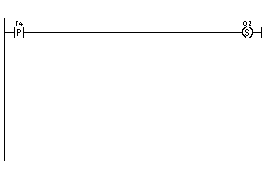
\includegraphics[scale=1.8]
  {textures/images/equations/eq1.pdf}
  \caption{Équation n°1}
  \label{fig:eq1}
\end{figure}


\subsubsection{Équation n°2- Éteindre LED Q2 \textit{(En service)}}
\label{sec:eq2}

Lorsqu'on active le bouton poussoir I5, que les LED Q1 ou Q8 sont allumées, on éteint Q2.

\begin{figure}[ht]
  \centering
  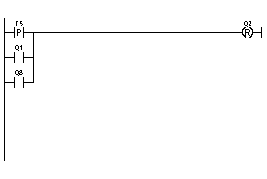
\includegraphics[scale=1.8]
  {textures/images/equations/eq2.pdf}
  \caption{Équation n°2}
  \label{fig:eq2}
\end{figure}


\subsubsection{Équation n°3- Allumer LED Q3 \textit{(Hors-service)}}
\label{sec:eq3}

Si Q2 est éteinte, alors on allume Q3.

\begin{figure}[ht]
  \centering
  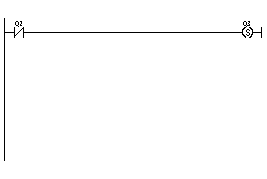
\includegraphics[scale=1.8]
  {textures/images/equations/eq3.pdf}
  \caption{Équation n°3}
  \label{fig:eq3}
\end{figure}


\subsubsection{Équation n°4- Éteindre LED Q3 \textit{(Hors-service)}}
\label{sec:eq4}

SI Q2 est allumée, alors on éteint Q3.

\begin{figure}[ht]
  \centering
  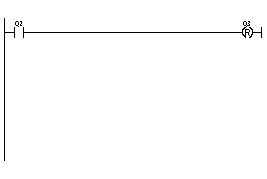
\includegraphics[scale=1.8]
  {textures/images/equations/eq4.pdf}
  \caption{Équation n°4}
  \label{fig:eq4}
\end{figure}

\newpage


\subsection{Gestion des lampes \textit{Défauts moteur}}
\label{sec:gestion-led-defaut}

\underline{\textbf{Énoncé :}} \guillemotleft \ \textit{La présence d'un défaut arrête totalement le fonctionnement de l'installation pour des raisons de sécurité.\\
Les lampes} Q1 \textit{et/ou} Q8 \textit{vont donner les alarmes de défaut liées, respectivement, au} moteur des convoyeurs d'évacuation \textit{et au} moteur principal. \guillemotright \

\subsubsection{Équation n°5- Allumer LED Q1 \textit{(Défaut Moteur des convoyeurs d'évacuation)}}
\label{sec:eq5}

Afin d'allumer la LED Q1, il faut que l'automate soit en service.\\
Il faut aussi que le moteur Q5 soit en surcharge, \textbf{ou}
que l'un des bits mémoires M11 et M12 soit à 1, \textbf{ou}, \textit{c'est un bonus}, que le moteur Q5 soit arrêté, mais qu'une boite passe le détecteur I3.

\begin{figure}[ht]
  \centering
  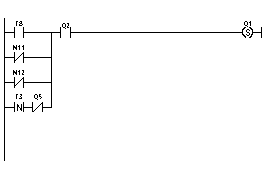
\includegraphics[scale=1.8]
  {textures/images/equations/eq5.pdf}
  \caption{Équation n°5}
  \label{fig:eq5}
\end{figure}


\subsubsection{Équation n°6- Allumer LED Q8 \textit{(Défaut Moteur principal)}}
\label{sec:eq6}

Afin d'allumer la LED Q8 il faut que le moteur Q4 soit en surcharge.

\begin{figure}[ht]
  \centering
  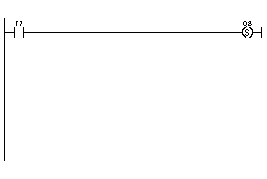
\includegraphics[scale=1.7]
  {textures/images/equations/eq6.pdf}
  \caption{Équation n°6}
  \label{fig:eq6}
\end{figure}

\newpage

\subsubsection{Équation n°7- Éteindre LED Q1 \textit{(Défaut Moteur des convoyeurs d'évacuation)}}
\label{sec:eq7}

Afin d'éteindre la LED Q1, il faut utiliser le \textbf{sélecteur à clé}, I6 \textit{(acquittement)}.

\begin{figure}[ht]
  \centering
  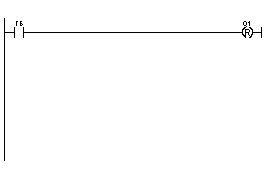
\includegraphics[scale=1.8]
  {textures/images/equations/eq7.pdf}
  \caption{Équation n°7}
  \label{fig:eq7}
\end{figure}


\subsubsection{Équation n°8- Éteindre LED Q8 \textit{(Défaut Moteur principal)}}
\label{sec:eq8}

Afin d'éteindre la LED Q8, il faut utiliser le \textbf{sélecteur à clé}, I6 \textit{(acquittement)}.

\begin{figure}[ht]
  \centering
  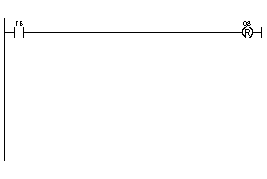
\includegraphics[scale=1.8]
  {textures/images/equations/eq8.pdf}
  \caption{Équation n°8}
  \label{fig:eq8}
\end{figure}

\newpage

\subsection{Encombrement des tapis d'évacuation}
\label{sec:encombrement}

\underline{\textbf{Énoncé :}} \guillemotleft \ \textit{Pour déterminer un encombrement, deux bits mémoires sont utilisés} M11 \textit{et} M12.\\
\textit{Pour} M11 \textit{par exemple, il est activé quand on veut pousser une boite, mais qu'une autre est présente sur le tapis d'évacuation.\\
Il est désactivé quand on a} I13. \guillemotright \

\subsubsection{Équation n°9- Désactivation du bit mémoire M11 \textit{(Vérin A)}}
\label{sec:eq9}

Afin de désactiver le bit mémoire M11 \textit{(bit à 0)}, il faut que I13 ne détecte pas de boite.

\begin{figure}[ht]
  \centering
  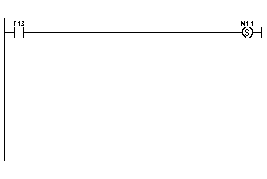
\includegraphics[scale=1.75]
  {textures/images/equations/eq9.pdf}
  \caption{Équation n°9}
  \label{fig:eq9}
\end{figure}


\subsubsection{Équation n°10- Activation du bit mémoire M11 \textit{(Vérin A)}}
\label{sec:eq10}

Pour l'activer \textit{(bit à 1)}, I13 doit détecter un boite et le \textbf{détecteur} I1 doit être en front descendant \textit{(c'est-à-dire qu'une boite détectée sort du champ du détecteur et se retrouve devant le vérin)}.

\begin{figure}[ht]
  \centering
  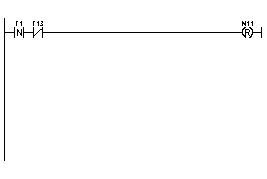
\includegraphics[scale=1.75]
  {textures/images/equations/eq10.pdf}
  \caption{Équation n°10}
  \label{fig:eq10}
\end{figure}

\newpage

\subsubsection{Équation n°11- Désactivation du bit mémoire M12 \textit{(Vérin B)}}
\label{sec:eq11}

Afin de désactiver le bit mémoire M12 \textit{(bit à 0)}, il faut que I14 ne détecte pas de boite \textit{(c'est-à-dire que le tapis d'évacuation n'est pas encombré)}.

\begin{figure}[ht]
  \centering
  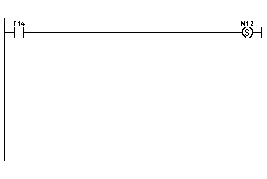
\includegraphics[scale=1.8]
  {textures/images/equations/eq11.pdf}
  \caption{Équation n°11}
  \label{fig:eq11}
\end{figure}


\subsubsection{Équation n°12- Activation du bit mémoire M12 \textit{(Vérin B)}}
\label{sec:eq12}

Pour l'activer \textit{(bit à 1)}, le \textbf{détecteur} I2 doit être en front descendant  et I14 doit détecter un boite.

\begin{figure}[ht]
  \centering
  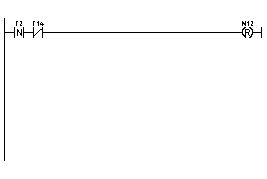
\includegraphics[scale=1.8]
  {textures/images/equations/eq12.pdf}
  \caption{Équation n°12}
  \label{fig:eq12}
\end{figure}

\newpage

\subsection{Gestion des vérins}
\label{sec:verins}

\underline{\textbf{Énoncé :}} \guillemotleft \ \textit{La sortie du vérin s'effectue soit en fin d'encombrement} (il faut pousser la boite encore présente), \textit{soit quand une boite est reconnue et qu'on n'a pas d'encombrement.\\
La tige du vérin doit être rentrée quand on est} Hors-service \textit{ou que la boite est positionnée sur son tapis d'évacuation}. \guillemotright \

\subsubsection{Équation n°13- Activation du moteur Q6 \textit{(Vérin A)}}
\label{sec:eq13}

Pour activer le moteur Q6, il faut que l'automate soit actif.\\
De plus, I1 doit être en front descendant et le bit mémoire M11 doit être à \textit{0}.

\begin{figure}[ht]
  \centering
  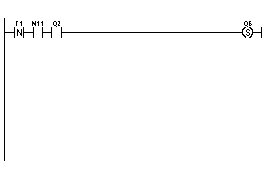
\includegraphics[scale=1.8]
  {textures/images/equations/eq13.pdf}
  \caption{Équation n°13}
  \label{fig:eq13}
\end{figure}


\subsubsection{Équation n°14- Désactivation du moteur Q6 \textit{(Vérin A)}}
\label{sec:eq14}

Pour que le vérin A soit désactivé, il faut que I13 détecte une boite, \textbf{ou} que l'automate soit éteint.

\begin{figure}[ht]
  \centering
  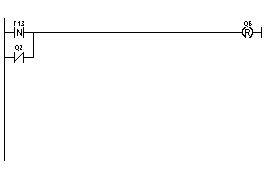
\includegraphics[scale=1.8]
  {textures/images/equations/eq14.pdf}
  \caption{Équation n°14}
  \label{fig:eq14}
\end{figure}

\newpage

\subsubsection{Équation n°15- Activation du moteur Q7 \textit{(Vérin B)}}
\label{sec:eq15}

Pour activer le moteur Q7, il faut que l'automate soit actif.\\
De plus, I2 doit être en front descendant et le bit mémoire M12 doit être à \textit{0}.

\begin{figure}[ht]
  \centering
  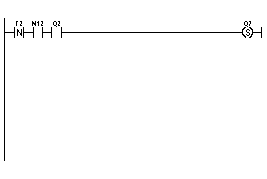
\includegraphics[scale=1.8]
  {textures/images/equations/eq15.pdf}
  \caption{Équation n°15}
  \label{fig:eq15}
\end{figure}


\subsubsection{Équation n°16- Désactivation du moteur Q7 \textit{(Vérin B)}}
\label{sec:eq16}

Pour que le vérin B soit désactivé, il faut que I14 détecte une boite, \textbf{ou} que l'automate soit éteint.

\begin{figure}[ht]
  \centering
  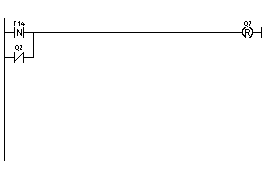
\includegraphics[scale=1.8]
  {textures/images/equations/eq16.pdf}
  \caption{Équation n°16}
  \label{fig:eq16}
\end{figure}

\newpage

\subsection{Gestion des moteurs des convoyeurs}
\label{sec:moteurs}

\underline{\textbf{Énoncé :}} \guillemotleft \ \textit{Le convoyeur principal fonctionne si les vérins sont rentrés, s'il n'y a pas de bourrage et si on est} En service.\\
\textit{Le moteur des tapis d'évacuation est en marche avec le sélecteur et la lampe} En service. \guillemotright \

\subsubsection{Équation n°17- Moteur principal \textit{(Q4)}}
\label{sec:eq17}

Le moteur principal est activé lorsque l'automate est en service et que les deux vérins sont rentrés.

\begin{figure}[ht]
  \centering
  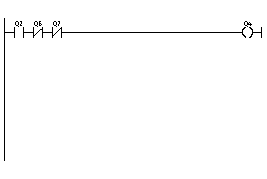
\includegraphics[scale=1.8]
  {textures/images/equations/eq17.pdf}
  \caption{Équation n°17}
  \label{fig:eq17}
\end{figure}


\subsubsection{Équation n°18- Moteur d'évacuation \textit{(Q5)}}
\label{sec:eq18}

Le moteur des convoyeurs d'évacuation est activé si l'automate est activé et que l'\textbf{interrupteur} I17 l'est aussi.

\begin{figure}[ht]
  \centering
  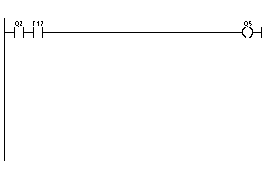
\includegraphics[scale=1.8]
  {textures/images/equations/eq18.pdf}
  \caption{Équation n°18}
  \label{fig:eq18}
\end{figure}

\newpage

\subsection{Gestion des compteurs de boites}
\label{sec:compteurs}

\underline{\textbf{Énoncé :}} \guillemotleft \ \textit{À la détection d'une boite grise par le capteur }I1, \textit{le} Vérin A \textit{pousse la boite sur le} convoyeur d'évacuation.\\
\textit{Un} compteur \textit{s'incrémente, indiquant le nombre de boites.\\
Un} compteur \textit{différent est utilisé pour chaque modèle de boite.\\
De plus, les compteurs doivent se réinitilaliser lors de l'activation du sélecteur à clé} I18. \guillemotright \

\subsubsection{Équation n°19- Compteur de boites \textit{(couleur Argent)}}
\label{sec:eq19}

Le \textbf{compteur} C1, pour les boites argentées, s'incrémente lorsque I13 détecte une boite.\\
Il se réinitialise si l'automate s'éteint, \textbf{ou} qu'on active le \textbf{sélecteur à clé}, I18.

\begin{figure}[ht]
  \centering
  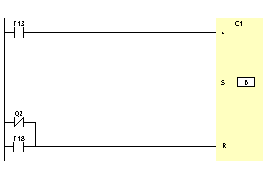
\includegraphics[scale=1.8]
  {textures/images/equations/eq19.pdf}
  \caption{Équation n°19}
  \label{fig:eq19}
\end{figure}


\subsubsection{Équation n°20- Compteur de boites \textit{(couleur Cuivre)}}
\label{sec:eq20}

Le \textbf{compteur} C2, pour les boites cuivrées, fonctionne de la même manière que le compteur C1.\\
La différence est que l'incrémentation est lancée lorsque \textbf{I14} détecte une boite.


\subsubsection{Équation n°21- Compteur de boites \textit{(couleur Or)}}
\label{sec:eq21}

Le \textbf{compteur} C3, pour les boites dorées, fonctionne de la même manière que les compteurs C1 et C2.\\
La différence est que l'incrémentation est lancée lorsque \textbf{I3} détecte une boite.

\newpage
\section{Conclusion}
\label{sec:conclusion}


\subsection{Résultat}
\label{sec:resultat}

L'automate trie les boites d'après leur couleur \textit{(argent, cuivre et or)}.\\

Lorsqu'il est à l'arrêt, la lampe \textit{Hors-service} est allumée, et la lampe \textit{En service} est éteinte. \\

L'appui sur le bouton poussoir  \guillemotleft \ \textbf{Start} \guillemotright \ allume la lampe \textit{En service}, éteint la lampe \textit{Hors-service} et met en route le moteur du convoyeur principal.\\
Sauf dans le cas où un défaut moteur a été détecté, ce qui arrêterait \textit{totalement} le fonctionnement de l'automate.\\
Celui-ci devra d'abord être corrigé afin de désactiver l'alarme lumineuse par un acquittement à l'aide du sélecteur à clé \textbf{I16}. Le moteur pourra alors être mis en route.\\

Pour mettre en marche le moteur des convoyeurs d'évacuation, le sélecteur \textbf{I17} doit être enclenché.\\
S'il n'est pas enclenché, un défaut moteur sera levé et affiché par la lampe \textbf{Q1}. Voici les différents cas qui lèveront le défaut :

\begin{itemize}
    
    \item le cas du défaut au moteur principal, c'est le cas le plus simple.\\
    Le moteur se retrouve en surcharge, ce qui enclenche l'arrêt d'urgence.
    
    \item le cas du défaut au moteur des convoyeurs d'évacuation, divisé en différents cas.
    
    \begin{itemize}
    
        \item le cas simple, le moteur est en surcharge, ce qui enclenche l'arrêt d'urgence.
        
        \item le cas de l'encombrement des tapis d’évacuation.\\
        Il est levé lorsqu'une boite est sous le détecteur du tapis d'évacuation, et qu'une autre \textit{(du même type)} se retrouve devant le vérin.\\
        C'est le cas lorsque le moteur des tapis d’évacuation est à l'arrêt.
        
        \item le cas \textit{bonus}, les tapis d'évacuation sont stoppés, mais le moteur principal ne l'est pas.\\
        Lorsqu'une boite est détectée par le dernier détecteur, \textbf{I3}, un défaut est levé.\\
        Sans ce dernier cas, la boite tomberait du tapis.
        
    \end{itemize}
    
\end{itemize}

\newpage

Lorsqu'une boite argentée ou cuivrée est repérée par le détecteur idoine, le moteur principal s'arrête et le vérin place la boite sur le tapis d'évacuation approprié.\\
Le vérin se replace et le moteur principal se relance une fois que la boite est détectée sur son tapis d'évacuation.\\
À ce moment, le compteur qui lui est lié s'incrémente de un.\\

Pour les boites dorées, il n'y a pas de vérin, donc pas d'arrêt du moteur principal.\\
En effet, une fois arrivées au bout du tapis principal, les boites se retrouvent sur le tapis d'évacuation correct s'il est activé.\\
C'est alors le dernier détecteur, \textbf{I3}, qui incrémente le compteur adéquat.\\

Les compteurs sont réinitialisés dans deux cas :

\begin{itemize}
    
    \item premier cas, l'automate est stoppé par le bouton poussoir \guillemotleft \ \textbf{Stop} \guillemotright.
    
    \item second et dernier cas, le sélecteur à clé, \textbf{I18}, est activé afin de réinitialiser les compteurs à la main.
    
\end{itemize}

\newpage
\newpage
\thispagestyle{empty}
\setcounter{page}{0}
\null
\newpage
\end{document}
